\def\panelWidth{1.75}
\def\panelHeight{1.25}

\def\panelBtwX{0.25}
\def\panelBtwY{0.25}

\def\panelPadX{0.375}
\def\panelPadY{0.375}

\def\panelBoardBvlX{0.5}
\def\panelBoardBvlY{0.5}

\def\panelBoardWidth{4}
\def\panelBoardHeight{1}

\def\panelPinHoleThickness{0.07}

\ctikzsubcircuitdef{spicpanel} {
    vcc, gnd,
    origin%
} {
    coordinate (#1-origin)
    ++(
    {((2*\panelPadX)+(2*\panelBtwX)+(3*\panelWidth))/2},
    %% {((2*-\panelPadY)-(\panelBtwY)-(2*\panelHeight))/2}
    -{((2*\panelPadY)+(\panelBtwY)+(2*\panelHeight)+\panelBoardHeight)/2}
    )
    node [inner sep = 0pt, anchor = center] {
        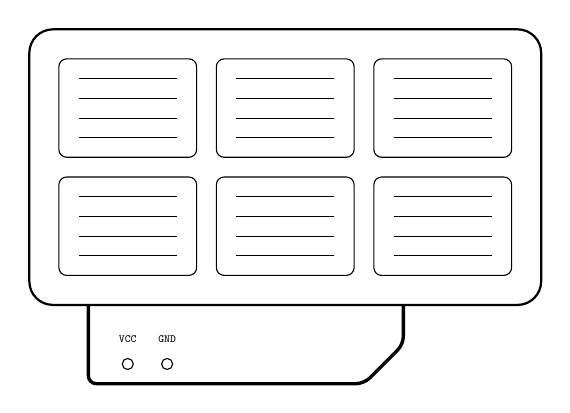
\begin{tikzpicture}
            \draw [thick, rounded corners = 3mm]
            (0,0) coordinate (origin)
            (origin) rectangle
            ++(
            {(2*\panelPadX)+(2*\panelBtwX)+(3*\panelWidth)},
            {(2*-\panelPadY)+(-\panelBtwY)+(2*-\panelHeight)}
            )
            ;
            \draw
            (origin) ++(\panelPadX,-\panelPadY)
            coordinate (panelstartx)
            coordinate (panelstarty)
            ;
            \foreach \y in {1,2} {
                \foreach \x in {1,2,3} {
                    \foreach \z in {0.25,0.5,...,1.25} {
                        \draw [very thin]
                        (panelstartx) ++(0.25,-\z)
                        -- +({\panelWidth-(2*0.25)},0)
                        ;
                    }
                    \draw [rounded corners = 1mm]
                    (panelstartx) rectangle +(\panelWidth,-\panelHeight)
                    ++({\panelBtwX+\panelWidth},0)
                    coordinate (panelstartx)
                    ;
                }
                \draw
                (panelstarty) ++(0,{-\panelBtwY-\panelHeight})
                coordinate (panelstarty)
                coordinate (panelstartx)
                ;
            }
            \draw [very thick, rounded corners = 1mm]
            (origin) ++(
            0.75,
            {(2*-\panelPadY)+(-\panelBtwY)+(2*-\panelHeight)}
            )
            -- ++(0,-{\panelBoardHeight})
            -- ++({\panelBoardWidth-\panelBoardBvlX},0)
            -- ++(\panelBoardBvlX,\panelBoardBvlY)
            -- ++(0,{\panelBoardHeight-\panelBoardBvlY})
            ;
            %% outputs
            \draw
            (origin) ++(
            0.75,
            {(2*-\panelPadY)+(-\panelBtwY)+(2*-\panelHeight)}
            )
            ++(0.5,{-\panelBoardHeight+0.25})
            circle (\panelPinHoleThickness)
            node [above = 5pt, font = \tiny, scale = 0.8] {\texttt{VCC}}
            ++(0.5,0)
            circle (\panelPinHoleThickness)
            node [above = 5pt, font = \tiny, scale = 0.8] {\texttt{GND}}
            ;
        \end{tikzpicture}
    }
    (#1-origin)
    ++(
    0.75,
    {(2*-\panelPadY)+(-\panelBtwY)+(2*-\panelHeight)}
    )
    ++(0.5,-\panelBoardHeight) coordinate (#1-vcc)
    ++(0.5,0) coordinate (#1-gnd)
}

\ctikzsubcircuitactivate{spicpanel}
